%%% template.tex
%%%
%%% This LaTeX source document can be used as the basis for your technical
%%% paper or abstract. Regardless of the length of your document, the commands
%%% are all the same.
%%% 
%%% The "\documentclass" command is the first command in your file. If you want to 
%%% prepare a version of your article with line numbers - a "review" version - 
%%% include the "review" parameter:
%%%    \documentclass[review]{acmsiggraph}
%%%

\documentclass{acmsiggraph}

%%% Title of your article or abstract.

\title{Exemplar-Based Structure-Aware Procedural Synthesis}
\author{Submission \#00000}
% \author{Stephen N. Spencer\thanks{e-mail:spencer@cs.washington.edu}\\Chair, ACM SIGGRAPH Publications Committee}
\pdfauthor{Submission \#00000}

%%% Used by the ``review'' variation; the online ID will be printed on 
%%% every page of the content.
\TOGonlineid{45678}

% User-generated keywords.

\keywords{radiosity, global illumination, constant time}

% With the "\setcopyright" command the appropriate rights management text will be added
% to your document.

%\setcopyright{none}
%\setcopyright{acmcopyright}
%\setcopyright{acmlicensed}
\setcopyright{rightsretained}
%\setcopyright{usgov}
%\setcopyright{usgovmixed}
%\setcopyright{cagov}
%\setcopyright{cagovmixed}
%\setcopyright{rightsretained}

% The year of publication in the "\copyrightyear" command.

\copyrightyear{2016}

%%% Conference information, from the completed rights management form.
%%% The "\conferenceinfo" command has two parameters: 
%%%    - conference name
%%%    - conference date and location
%%% The "\isbn" field includes the year and month after the article ISBN.

\conferenceinfo{SIGGRAPH 2016 Posters}{July 24-28, 2016, Anaheim, CA} 
\isbn{978-1-4503-ABCD-E/16/07} 
\doi{http://doi.acm.org/10.1145/9999997.9999999}

\usepackage{overpic}
\usepackage{amssymb}
\usepackage{graphicx}
% \usepackage{microtype} %< better text layout

%%
%% colors
%% 
\usepackage{color}
\definecolor{turquoise}{cmyk}{0.65,0,0.1,0.3}
\definecolor{purple}{rgb}{0.65,0,0.65}
\definecolor{dark_green}{rgb}{0, 0.5, 0}
\definecolor{orange}{rgb}{0.8, 0.6, 0.2}
\definecolor{red}{rgb}{0.8, 0.2, 0.2}
\definecolor{blueish}{rgb}{0.0, 0.7, 1}
\definecolor{light_gray}{rgb}{0.7, 0.7, .7}
\definecolor{pink}{rgb}{1, 0, 1}

%%
%% markdown (needs "--shell-escape" in compiler options)
%% 
% \usepackage{markdown}

%%
%% general comments
%% 
\newcommand{\hide}[1]{{}} %< discards
\newcommand{\todo}[1]{{\color{red}#1}}
\newcommand{\TODO}[1]{{\color{red}[TODO: #1]}}
\newcommand{\revision}[1]{{\color{red}#1}}
\renewcommand{\revision}[1]{{#1}} %< disable

%%
%% environments
%% 
\newenvironment{draft}{\color{red}}{\color{black}}
\newenvironment{DRAFT}{\color{red}}{\ignorespacesafterend}

%%
%% personal comments
%% 
\newcommand{\AT}[1]{{\color{blueish}[AT: #1]}} % andrea comment
\newcommand{\at}[1]{{\color{blueish}#1}} % andrea edit
% \newcommand{\XX}[1]{{\color{turquoise}[XX: #1]}} % ??
% \newcommand{\XX}[1]{{\color{dark_green}[XX: #1]}} % ??
% \newcommand{\XX}[1]{{\color{orange}[XX: #1]}} % ??

%%
%% shortcut for references
%% 
\newcommand{\Fig}[1]{Figure~\ref{fig:#1}}
\newcommand{\Figure}[1]{Figure~\ref{fig:#1}}
\newcommand{\eq}[1]{(\ref{eq:#1})}
\newcommand{\Eq}[1]{Equation~\ref{eq:#1}}
\newcommand{\Equation}[1]{Equation~\ref{eq:#1}}
\newcommand{\Sec}[1]{Section~\ref{sec:#1}}
\newcommand{\Section}[1]{Section~\ref{sec:#1}}
\newcommand{\Appendix}[1]{Appendix~\ref{app:#1}}

%%
%% More macros
%%
\newcommand{\eg}{\emph{e.g.~}}
\newcommand{\ie}{\emph{i.e.~}}

%%
%% SHOW PATH OF INSERTED IMAGES
%% 
\usepackage{currfile}
\newcommand{\vertical}[1]{{\rotatebox{90}{#1}}}
\newcommand{\myfigurename}{\put(-3,0){\vertical{\todo{\currfiledir}}}}
% \renewcommand{\myfigurename}{} %< disables


%%
%% text layout (personally hate new SIGGRAPH template)
%%
% Insert whitespace at the end of a paragraph
\setlength{\parskip}{.5\baselineskip}%
% Don't intent by default on new paragraph
\setlength{\parindent}{0pt}%
\begin{document}
%%% This is the ``teaser'' command, which puts an figure, centered, below 
%%% the title and author information, and above the body of the content.
\teaser{
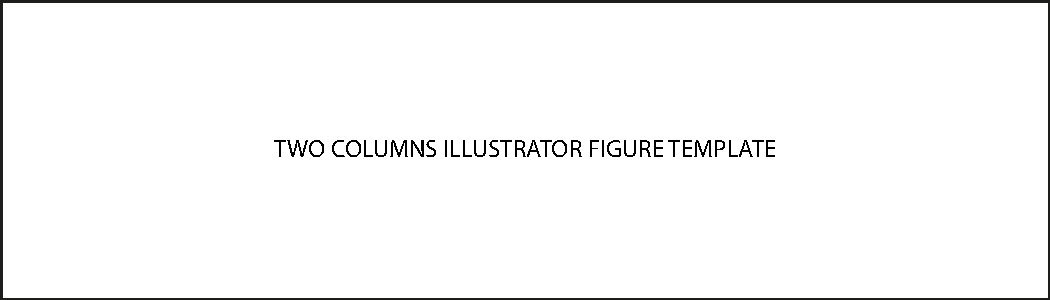
\includegraphics[width=\linewidth]{fig/teaser/item.pdf}
\caption{Spring Training 2009, Peoria, AZ.}
}

% \teaser{
% \includegraphics[width=\linewidth]{fig/teaser/composite.pdf}
% \centering
% \caption*{Our system tracks the motion of hands while remaining robust to fast motion, sensor imperfections and self-occlusions.}
% \label{fig:teaser}
% }
\maketitle
\begin{abstract}
\begin{draft}
Lorem ipsum dolor sit amet, consectetur adipisicing elit, sed do eiusmod tempor incididunt ut labore et dolore magna aliqua. Ut enim ad minim veniam, quis nostrud exercitation ullamco laboris nisi ut aliquip ex ea commodo consequat. Duis aute irure dolor in reprehenderit in voluptate velit esse cillum dolore eu fugiat nulla pariatur. Excepteur sint occaecat cupidatat non proident, sunt in culpa qui officia deserunt mollit anim id est laborum.
Lorem ipsum dolor sit amet, consectetur adipisicing elit, sed do eiusmod tempor incididunt ut labore et dolore magna aliqua. Ut enim ad minim veniam, quis nostrud exercitation ullamco laboris nisi ut aliquip ex ea commodo consequat. Duis aute irure dolor in reprehenderit in voluptate velit esse cillum dolore eu fugiat nulla pariatur. Excepteur sint occaecat cupidatat non proident, sunt in culpa qui officia deserunt mollit anim id est laborum.
\end{draft}
\end{abstract}
%
% The code below should be generated by the tool at
% http://dl.acm.org/ccs.cfm
% Please copy and paste the code instead of the example below. 
%
\begin{CCSXML}
<ccs2012>
<concept>
<concept_id>10010147.10010371.10010382</concept_id>
<concept_desc>Computing methodologies~Image manipulation</concept_desc>
<concept_significance>500</concept_significance>
</concept>
<concept>
<concept_id>10010147.10010371.10010382.10010236</concept_id>
<concept_desc>Computing methodologies~Computational photography</concept_desc>
<concept_significance>300</concept_significance>
</concept>
</ccs2012>
\end{CCSXML}

\ccsdesc[500]{Computing methodologies~Image manipulation}
\ccsdesc[300]{Computing methodologies~Computational photography}

%
% End generated code
%

% The next three commands are required, and insert the user-generated keywords, 
% The CCS concepts list, and the rights management text.
% Please make sure there is a blank line between each of these three commands.

\keywordlist

\conceptlist

\printcopyright
% !TEX root = ../htrack.tex

% Things to include in the intro are (not necessarily in this order):
% 
% Problem Statement: What's the problem you want to solve?
% 
% Motivation: Why is this an interesting problem? Who cares about it? Why now? Why is it appropriate for the conference audience?
% 
% Research Gap, Novelty: Why is new research required? Why can the problem not be solved with existing methods? How does the proposed solution differ from and/or improve upon existing work?
% 
% Technical Contribution: What's the key technical idea to solve the problem? Why is it beautiful?
% 
% Applications / Future Work: What will your solution enable? How does it project into the future? How will it inspire future work?

\section{Introduction}
Lorem ipsum dolor sit amet, consectetur adipisicing elit, sed do eiusmod tempor incididunt ut labore et dolore magna aliqua. Ut enim ad minim veniam, quis nostrud exercitation ullamco laboris nisi ut aliquip ex ea commodo consequat. Duis aute irure dolor in reprehenderit in voluptate velit esse cillum dolore eu fugiat nulla pariatur. Excepteur sint occaecat cupidatat non proident, sunt in culpa qui officia deserunt mollit anim id est laborum.

\AT{This is what I've been using in many groups to do inline annotations}. See the tweaks.tex file to know what is your id (GM, AT, NP, PC, EP), for example, for giorgio: \GM{ciao ciao!!}.

\begin{figure}[t]
\centering
\begin{overpic} 
% [width=\linewidth]
[width=\linewidth,grid,tics=10]
{\currfiledir/item.pdf}
\put(10,10){\todo{\currfiledir}}
\end{overpic}
\caption{\todo{\currfiledir}}
\label{fig:onecol}
\end{figure}
% \filename@parse{path/to/file.c}
\section{Related Work}
\label{sec:related}

You can cite by name with \citeN{htrack}, or in standard way with \cite{sparseicp}.
\begin{draft}
Lorem ipsum dolor sit amet, consectetur adipisicing elit, sed do eiusmod tempor incididunt ut labore et dolore magna aliqua. Ut enim ad minim veniam, quis nostrud exercitation ullamco laboris nisi ut aliquip ex ea commodo consequat. Duis aute irure dolor in reprehenderit in voluptate velit esse cillum dolore eu fugiat nulla pariatur. Excepteur sint occaecat cupidatat non proident, sunt in culpa qui officia deserunt mollit anim id est laborum
\end{draft}

% \clearpage %< DOES NOT WORK
\begin{figure*}[t]
\centering
\begin{overpic} 
[width=\linewidth]
% [width=\linewidth,grid,tics=10]
{\currfiledir/item.pdf}
\myfigurename{}
\end{overpic}
\caption{
% 
Template for a two column figure.
% 
}
% \label{fig:}
\end{figure*}

\begin{figure}[t]
\centering
\begin{overpic} 
[width=\linewidth]
% [width=\linewidth,grid,tics=10]
{\currfiledir/item.pdf}
\myfigurename{}
\end{overpic}
% \caption{}
% \label{fig:}
\end{figure}

\section{Overview}
\begin{draft}
Lorem ipsum dolor sit amet, consectetur adipisicing elit, sed do eiusmod tempor incididunt ut labore et dolore magna aliqua. Ut enim ad minim veniam, quis nostrud exercitation ullamco laboris nisi ut aliquip ex ea commodo consequat. Duis aute irure dolor in reprehenderit in voluptate velit esse cillum dolore eu fugiat nulla pariatur. Excepteur sint occaecat cupidatat non proident, sunt in culpa qui officia deserunt mollit anim id est laborum.
\end{draft}
\section{Technical section}
\label{sec:technical}
Lorem ipsum dolor sit amet, consectetur adipisicing elit, sed do eiusmod tempor incididunt ut labore et dolore magna aliqua. Ut enim ad minim veniam, quis nostrud exercitation ullamco laboris nisi ut aliquip ex ea commodo consequat. Duis aute irure dolor in reprehenderit in voluptate velit esse cillum dolore eu fugiat nulla pariatur. Excepteur sint occaecat cupidatat non proident, sunt in culpa qui officia deserunt mollit anim id est laborum.
\section{Evaluation}
\label{sec:eval}
Lorem ipsum dolor sit amet, consectetur adipisicing elit, sed do eiusmod tempor incididunt ut labore et dolore magna aliqua. Ut enim ad minim veniam, quis nostrud exercitation ullamco laboris nisi ut aliquip ex ea commodo consequat. Duis aute irure dolor in reprehenderit in voluptate velit esse cillum dolore eu fugiat nulla pariatur. Excepteur sint occaecat cupidatat non proident, sunt in culpa qui officia deserunt mollit anim id est laborum. Lorem ipsum dolor sit amet, consectetur adipisicing elit, sed do eiusmod tempor incididunt ut labore et dolore magna aliqua. Ut enim ad minim veniam, quis nostrud exercitation ullamco laboris nisi ut aliquip ex ea commodo consequat. Duis aute irure dolor in reprehenderit in voluptate velit esse cillum dolore eu fugiat nulla pariatur. Excepteur sint occaecat cupidatat non proident, sunt in culpa qui officia deserunt mollit anim id est laborum.


\section{Conclusions}

Lorem ipsum dolor sit amet, consectetur adipisicing elit, sed do eiusmod tempor incididunt ut labore et dolore magna aliqua. Ut enim ad minim veniam, quis nostrud exercitation ullamco laboris nisi ut aliquip ex ea commodo consequat. Duis aute irure dolor in reprehenderit in voluptate velit esse cillum dolore eu fugiat nulla pariatur. Excepteur sint occaecat cupidatat non proident, sunt in culpa qui officia deserunt mollit anim id est laborum.

\paragraph*{Limitations.}
Lorem ipsum dolor sit amet, consectetur adipisicing elit, sed do eiusmod tempor incididunt ut labore et dolore magna aliqua. Ut enim ad minim veniam, quis nostrud exercitation ullamco laboris nisi ut aliquip ex ea commodo consequat. Duis aute irure dolor in reprehenderit in voluptate velit esse cillum dolore eu fugiat nulla pariatur. Excepteur sint occaecat cupidatat non proident, sunt in culpa qui officia deserunt mollit anim id est laborum.

\paragraph*{Future Work.}
Lorem ipsum dolor sit amet, consectetur adipisicing elit, sed do eiusmod tempor incididunt ut labore et dolore magna aliqua. Ut enim ad minim veniam, quis nostrud exercitation ullamco laboris nisi ut aliquip ex ea commodo consequat. Duis aute irure dolor in reprehenderit in voluptate velit esse cillum dolore eu fugiat nulla pariatur. Excepteur sint occaecat cupidatat non proident, sunt in culpa qui officia deserunt mollit anim id est laborum.
\section*{Acknowledgements}
To Robert, for all the bagels.
\bibliographystyle{acmsiggraph}
\bibliography{paper}
\end{document}
